\documentclass[final]{anthology-ch}

\usepackage{booktabs}
\usepackage{graphicx}

\title{How `Pagan' Is My Text? Information Extraction from Untranscribed Data}

\author[1,2]{Rachael M. Griffiths}[orcid=0000-0003-1381-0718]

\author[1]{Marieke Meelen}[
orcid=0000-0003-0395-8372
]

\affiliation{1}{DTAL, University of Cambridge, United Kingdom}
\affiliation{2}{EPHE-PSL, Paris, France}

\keywords{HTR, Information Extraction, Text Classification, Tibetan, Religious Studies}

\pubyear{2025}
\pubvolume{3}
\pagestart{1246}
\pageend{1257}
\conferencename{Computational Humanities Research 2025}
\conferenceeditors{Taylor Arnold, Margherita Fantoli, and Ruben Ros}
\doi{10.63744/aYiz0uLyIS4f}
\paperorder{76}

\addbibresource{bibliography.bib}

\begin{document}

\maketitle

\begin{abstract}
In this paper, we present our work-in-progress on Information Extraction and Text Classification from large manuscript collections that have not yet been transcribed. We propose a three-stage
pipeline starting with  digitisation using a collaborative Handwritten Text Recognition
(HTR) workflow, followed by Normalisation and Segmentation of the texts to
create searchable collections, and, finally, we discuss how Text Classification
and Information Extraction can help us identify the texts with Tibetan `Pagan' religious features that are hidden among texts that belong to the Buddhist and B\"on religious traditions.
\end{abstract}

\section{Introduction}
\label{sec:intro}

In the 7th century CE Buddhism was introduced to Tibet as part of a grand imperial project, and it became the official national religion in the 8th. This seems to have had little impact on the autochthonous `Pagan' religious practices: there were still animal sacrifices at royal funerals \cite{Aldenderfer13} and there were no monks but instead a class of hereditary priests to revere the Tibetan king \cite{berounskyramble}. To distinguish itself from Pagan cults, one religious school identified themselves more specifically as Yungdrung (``Eternal'') B\"on. Yungdrung B\"on is still practised by 2-5\% of Tibetans to this day \cite{Baumer2002}. This religion contains much that resembles Buddhist belief and practice. Like Buddhism, B\"on has a very rich scriptural tradition. However, some of the B\"on texts concern beliefs and practices that are clearly unrelated to Buddhism: these contain traces of the Pagan traditions that were suppressed by the Buddhist authorities during the imperial period. Until recently, almost all we knew about these pre-Buddhist Pagan traditions comes from Old Tibetan texts discovered in a cave at Dunhuang, on the Silk Road, or hidden, older elements in canonical B\"on texts.

In 2005, however, a large number of manuscripts (over 75,000 pages) constituting the ritual repertoire of a class of priests, called Leyu, was discovered in the Sino-Tibetan borderlands.\footnote{Facsimiles of some of these manuscripts have been published in collections. For more information on the discovery and publication of these manuscripts, see \cite{berounskyramble}.} Preliminary investigations of facsimiles suggest that these texts contain genuinely archaic non-Buddhist rituals and narratives closely resembling those of the early Pagan sources. In addition, further collections (containing at least another 25,000 pages) have been identified in B\"on villages in Dolpo and Mustang (Nepal), among the indigenous Baima communities in Sichuan and Gansu (China), and in manuscripts recovered from the Dunhuang caves and in the Gathang Bumpa stupa, southern Tibet \cite{berounskyramble}. These collections have the potential to form an invaluable resource to uncover the myths, ritual practices and worldview of the oldest religion of Tibet, but there are major challenges to overcome before we can reconstruct the features that can give us a comprehensive understanding of these Pagan religious practices. First of all, the collections contain a large amount of Buddhist and B\"on texts. In the latter, we often find parts of myths or rituals that go back to ancient Pagan traditions, but these are not marked in any way. Second, the manuscripts are not yet transcribed, and manually producing transcriptions is difficult due to the extremely challenging continuous (i.e. without word breaks) Tibetan \textit{ume} script full of complex abbreviations and non-standard spellings.

In this paper, we therefore first focus on the crucial question of how to find the `Pagan' religious features in this vast amount of extremely difficult and untranscribed data. We propose a three-stage pipeline. Stage 1 involves the digitisation process, using a collaborative Handwritten Text Recognition (HTR) workflow (Section \ref{sec:htr}). Stage 2 consists of Normalisation and Segmentation of texts to create searchable collections (Section \ref{sec:normseg}). Finally, in Section \ref{sec:textclass}, we discuss how Text Classification and Information Extraction can help us identify the Pagan texts and sections that are hidden among the Buddhist and B\"on materials.

\begin{figure}[h!]
\centering
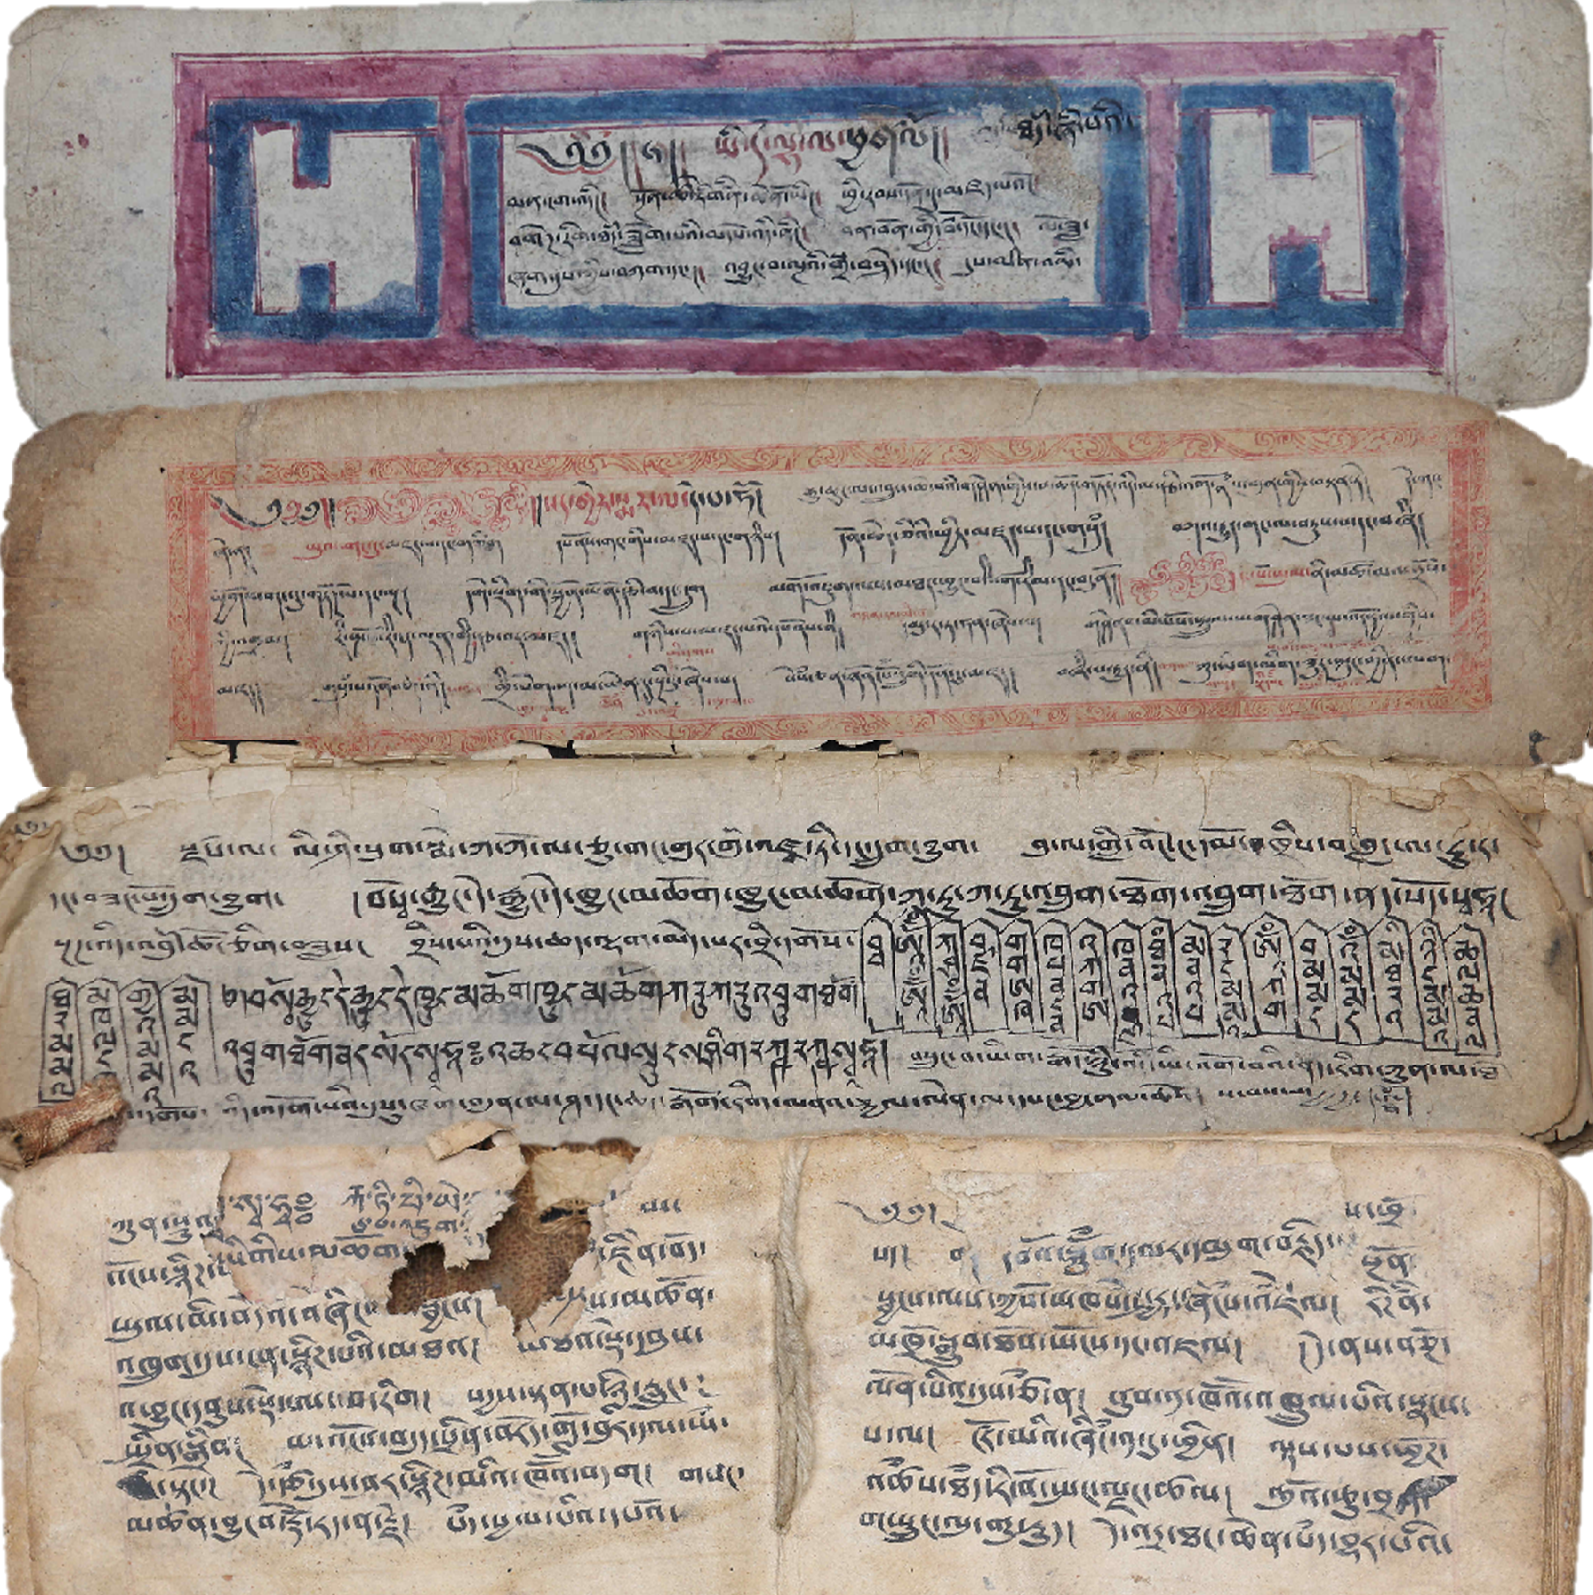
\includegraphics[width=1\linewidth]{figures/PaganTibetCorpus.png}
\caption{Sample of the diverse newly-discovered Tibetan corpus.}
\label{fig:corpus}
\end{figure}

\section{Handwritten Text Recognition} \label{sec:htr}

\noindent In order to maximise our efficiency with limited time and funding, we have developed a collaborative workflow that utilises the strengths of all participants.\footnote{The potential benefits of leveraging collective expertise to enhance the accuracy and accessibility of HTR projects have been discussed in recent scholarship on collaborative or crowdsourced transcription workflows, such as \cite{andersdotterSecretariesWorkAccessing2022}, \cite{Transkribusworkflow}, and \cite{tarride2023handwritten}.} The script in which most of these collections are written is a difficult form of Tibetan \textit{ume} or `headless' script, which only a handful of expert philologists and some Tibetan B\"on monks can read. Figure \ref{fig:corpus} shows a sample of this diverse corpus. In addition to the challenges posed by the script and text format (horizontal Tibetan pecha style, developed from Indian palm leaf manuscripts), the language itself reflects a non-standard variety of Tibetan, with unorthodox spellings and mixed with local, non-Tibetan words and graphemes/symbols. In addition to these philological challenges, the vast amount of data raises questions about both short- and long-term storage. To resolve these issues, we collaborate with international experts in Tibetan philology (both internal and external),\footnote{The external experts are monks from the Triten Norbutse Institute (TNI) in Kathmandu.} data storage (the online BDRC library, who will make our eTexts publicly available),\footnote{The Buddhist Digital Resource Centre: \url{https://www.bdrc.io/buda-archive/}} as well as programmers from Esukhia, a Tibetan tech and education charity based in Dharamsala.\footnote{\url{https://esukhia.net/}} Figure \ref{fig:htr-workflow} shows this workflow (see \cite{meelengriffiths2025} for further details on the HTR workflow).

\begin{figure}[h!]
\centering
\includegraphics[width=0.95\linewidth]{figures/workflow2.png}
\caption{Collaborative HTR workflow.}
\label{fig:htr-workflow}
\end{figure}

\subsection{Creating Ground Truth}
\label{sec:creatingGT}

\noindent As the internal HTR team, we first select a diverse batch of images with different forms of Tibetan \textit{ume} scripts (see sample in Fig. \ref{fig:corpus}). We then divide this into two separate batches: a `manual input' batch and a `correction' batch. Both batches are uploaded and backed up on the BDRC servers, and are also uploaded to a custom-made tool created by Esukhia for inputting and correcting transcriptions (shown in Fig. \ref{fig:manual-pechatools}).

\begin{figure}
\centering
\includegraphics[width=0.95\linewidth]{figures/openpecha1.png}
\caption{Screenshot of the final-reviewing page (i.e. third check) of manual input tasks.}
\label{fig:manual-pechatools}
\end{figure}

Each batch is assigned to a specific transcription team. The `manual team' (`Team A' in Fig. \ref{fig:htr-workflow}) consists of four TNI monks who are given `manual input' batches to transcribe manually. The `correction' batches undergo a different process. These are first transcribed automatically using the  Tibetan \textit{ume} models created by the TibSchol project in Vienna,\footnote{The Dawn of Tibetan Scholasticism (11th–13thc.) (H2020-Cog-101001002) \url{https://cordis.europa.eu/project/id/101001002/reporting}.
The HTR models trained by the TibSchol project were the only ones available in January 2024. Since then, the BDRC has developed an OCR app that includes \textit{ume} models. For a discussion of this app and its suitability for the manuscripts presented here, see \cite{meelengriffiths2025}.} which are available through the Transkribus platform \cite{Griffiths2024}.\footnote{\url{www.transkribus.org}} Although the Ground Truth that formed the basis of these HTR models also consists of Tibetan \textit{ume} texts, the quality of the images used are generally better and the handwriting is much clearer and more regular than our collections.\footnote{Samples of the images from the TibSchol Ground Truth can be found in \cite{hugon2024} and \cite{Griffiths2024}.} Consequently, the resulting transcriptions contain a high number of errors (over 60\% on average), which require extensive manual correction. The output from the TibSchol HTR model is uploaded alongside the images from the `correction' batches, which is then corrected by the `correction team' (`Team B' in Fig. \ref{fig:htr-workflow}), consisting of four TNI monks. The transcriptions produced by both teams then undergo two rounds of review: firstly by the TNI team leaders, and then a final review by the internal HTR team.

To help both teams create diplomatic transcriptions, the internal team prepared a transcription manual \cite{meelengriffiths2025b} and cheat sheet \cite{griffithsmeelen2025a} with examples of the most challenging cases, e.g. Chinese or other non-Tibetan characters and symbols (see. Fig. \ref{fig:normalisation}). Creating these guidelines for purely diplomatic transcriptions was essential due to the difficult nature of the source material and the general tendencies of the TNI monks to `interpret' and therefore normalise the text by adding expanded forms and fixing spellings. While Normalisation is eventually essential for downstream NLP tasks (see Section \ref{sec:normseg} below), the haphazard nature of `corrections' at this stage poses issues.

For example, any form of Normalisation brings the transcription further away from the original manuscript text. This creates issues for training new HTR models as the transcriptions no longer directly correspond to the images. If abbreviations were consistent this would not be a problem, but there is major variation in scribal conventions across these collections. Losing this variation essentially means losing philological features that can help us try to establish the date and place of origin of the individual texts, which will be of crucial importance for establishing how Pagan traditions were connected and possibly spread to different parts of Tibet and its borderlands. We therefore first focus on diplomatic transcriptions that resemble the original manuscripts as accurately as possible.

\subsection{HTR training \& results}
\label{sec:htrtraining}

All transcriptions are triple-checked (by two TNI monks and one internal expert) to ensure high-quality data that will be used as Ground Truth for training HTR models. These enhanced checks slow down the process, but the difficulty of the source material requires this: after only one or two checks, 10-15\% of errors typically remained. If such a high error rate is embedded in the Ground Truth, the overall accuracies drop to the extent that models become unusable for transcribing new images.

Since the Ground Truth used for the TibSchol HTR \textit{ume} models differs from our collections,\footnote{The TibSchol models were trained on c. 500 pages of \textit{ume} script from a corpus of Tibetan Buddhist scholastic literature written between the 11th and 14th centuries. Most of the images are black-and-white scans. Transcriptions are diplomatic - although most punctuation is omitted or simplified - and use the Wylie transliteration system \cite{Wylie59} in Roman script \cite{hugon2024}.} we incrementally trained new models - using  the Transkribus platform - based on 490, 900, and 1200 triple-checked pages from our collections.\footnote{Two of these models have already been made publicly available on Transkribus: `PaganTibet Ume 1' (Transkribus ID: 131553) and `PaganTibet Ume 2' (Transkribus ID: 193821). The Ground Truth is deposited on Zenodo \cite{griffithsetal2025_ume1+2GT}.} Each iteration contained a wide variety of training data from collections found in Dolpo and Mustang in Nepal, as well as along the Sino-Tibetan borderlands, representing different image quality, scribal practices, and orthographic conventions (if any). Because of the diversity of these training sets, the resulting models perform much better on our diverse collections than the TibSchol HTR models.\footnote{The TibSchol models produce output in Wylie transliteration, which poses accessibility challenges for our downstream applications. Because we chose to produce transcriptions in Tibetan Unicode, the TibSchol models could not serve as a base model.} Testing on two randomly selected texts that were not part of the Ground Truth, the Tibschol HTR model has an average error rate of 59.79\%,\footnote{We used the model `Tibetan Cursive (Drutsa)' (Transkribus ID: 176765), as its script style better corresponds to our manuscript material than `Tibetan Cursive (Betsug)'
(Transkribus ID: 54935).} whereas the new models trained on 490 and 900 pages already show an improvement with error rates of 23.45\% and 12.74\% respectively \cite{griffithsmeelen2025a}. Because of this, later `correction' batches for the external HTR team were processed with these newer models to improve the overall results. After completing 2,000 pages, the `manual input' team was switched to correction tasks, resulting in the creation of c. 30,000 pages of double-checked data in one year.

Character Error Rates (CER) on validation sets (we reserve 10\% of the overall triple-checked data for validation) still show variation (5-10\%), indicating that adding more Ground Truth remains worthwhile given the diversity of scribal practices across the collections.\footnote{See \cite{meelengriffiths2025} for a breakdown and analysis of HTR results.} We therefore estimate that with approximately 2,500 pages of triple-checked training data, the HTR model should perform well enough to process all remaining images in the collections and produce diplomatic transcriptions that preserve crucial philological variation. The following section discusses how these diplomatic transcriptions can be converted into searchable texts suitable for Information Extraction and Text Classification.

\section{Normalisation \& Segmentation} \label{sec:normseg}

As mentioned in Section \ref{sec:htr}, these collections are written in a challenging form of Tibetan that exhibits a variety of complex features not found in standard Classical Tibetan texts. While the diplomatic transcriptions are crucial for the preservation of philological and linguistic variation, they are not directly suitable for creating annotated corpora or any other downstream NLP tasks. In order to annotate the texts, the raw transcriptions need further preprocessing in the form of Normalisation and Word Segmentation before they can be analysed as searchable eTexts.

\subsection{Normalisation} \label{sec:norm}

Previous work on Normalisation of Tibetan has largely focused on converting Old Tibetan into a more standardised form of Classical / Written Tibetan \cite{faggionatomeelen2019developing}. Although this provides a useful starting point for handling certain archaic orthographical features, the Normalisation required for our diplomatic transcriptions is considerably more extensive, including splitting contracted forms, recognising and converting non-Tibetan characters, decoding abbreviations, and converting dialect features. Examples of these challenging features are shown in Fig. \ref{fig:normalisation}.

We therefore use an existing preprocessing script as a starting point \cite{faggionato-etal-2022-nlp},\footnote{\url{https://github.com/lothelanor/actib/blob/main/preprocessing.py}} but have extended it in two key ways.\footnote{Scripts developed for the HTR-to-Text Classification workflow are being made available at \url{www.github.com/pagantibet}} First, we expanded the set of standardisation rules to address the non-standard forms described above. Second, we built a preliminary abbreviation dictionary to enable the automatic expansion of contracted forms. These initial extensions, however, do not yet comprehensively cover all complex cases in the collections. To expand our dictionary and build on the existing preprocessing script, we use a collaborative workflow similar to that discussed in Section \ref{sec:htr}. Esukhia has also developed a custom-made tool to identify and normalise textual variants, shown in Fig. \ref{fig:normtool}, as well as a `Dictionary Correction' tool that allows expansions to be checked in context before they are added to the growing abbreviation dictionary.

\begin{figure}[h!]
\centering
\includegraphics[width=0.9\linewidth]{figures/normalisationex_NEW.png}
\caption{Examples of challenging cases of Normalisation. }
\label{fig:normalisation}
\end{figure}

\begin{figure}[h!]
\centering
\includegraphics[width=0.9\linewidth]{figures/normalisationtool.png}
\caption{Customised tool to normalise diplomatic transcriptions.}
\label{fig:normtool}
\end{figure}

\noindent After this manual correction stage, we apply a postprocessing script to resolve any remaining recurring issues, such as non-standard or double punctuation marks. The normalised text is then compared with the diplomatic version to identify new cases that can be added to the Normalisation rules and abbreviation dictionary. In this semi-supervised workflow, part of the corpus is manually checked twice, and the rest is processed automatically using optimised Normalisation rules.

\begin{figure}[h!]
\centering
\includegraphics[width=0.6\linewidth]{figures/Dip-vs-Norm2.png}
\caption{Example of diplomatic and normalised text.}
\label{fig:dipvsnorm}
\end{figure}

\subsection{Segmentation}
\label{sec:seg}

\noindent Since there are no word boundaries in the Tibetan script, Tokenisation is not a trivial task. Normalisation opens up the opportunity to use existing Segmentation tools  originally developed for Classical Written Tibetan. We therefore use an existing segmenter \cite{meelenhill:2017}, which reports a high level of accuracy (99\%) and is freely available and easy to use.\footnote{\url{https://github.com/lothelanor/actib}} An additional advantage of using this script is the ability to extend its output beyond Word Segmentation to include Sentence Segmentation and detailed morphosyntactic annotation. Both of these are valuable for further NLP tasks, which we turn to in the next section.

\section{How Pagan is my text?} \label{sec:textclass}

\noindent Once all collections are normalised and segmented, they can be compared with known Buddhist and B\"on canonical texts. When experts read individual texts, they can identify parts that contain Pagan features based on typical non-Buddhist and non-B\"on content, such as rituals involving animal sacrifice, fox fumigation, priests as mediators etc. Yet even when the language is more standardised, reading over 100,000 pages to identify which parts contain Pagan features is impossible. Focusing only on text titles would reduce the task, but titles do not always reflect the actual content or can be absent altogether. Furthermore, Pagan myths and rituals are often embedded within larger text that are otherwise part of the Buddhist or B\"on canon.

Therefore, even if all collections are easily searchable (i.e. transcribed, normalised, and segmented as discussed above), the specific question of how we can distinguish the Pagan (parts of) texts from the Buddhist and B\"on ones remains. In NLP terms, this question can be addressed through a combination of Information Extraction and Text Classification methods.

\subsection{Information Extraction} \label{sec:IE}

\noindent Extracting specific information from texts can be done in various ways. We make a distinction between philological or codicological features on the one hand, such as specific scribal practices and textual elements, and linguistic and content features on the other. Identifying Pagan features within our corpus requires extracting specific content elements that can be used to help differentiate traditions, including deity names, ritual practices, and specific terminology. We are pursuing this through two complementary approaches.

The first is through Title Extraction and Text Segmentation. As no comprehensive catalogue exists for our collections, we manually tag key features such as titles, images, and decorative elements, while preparing Ground Truth in Transkribus. Once finalised, these tags will be extracted from TEI exports to create a content catalogue and to segment the corpus into analysable units. However, titles alone often prove vague and unreliable indicators of content, necessitating more targeted feature extraction.

The second approach is through semi-supervised feature annotation. Esukhia has developed a custom annotation tool that enables both internal and external team members to annotate specific Pagan features within normalised texts. These manually annotated examples will serve as training data for future work that involves supervised Information Extraction focusing on Named Entities and Semantic Roles in the first instance. This approach will enable identification of Pagan passages and provide fine-grained searchability beyond categorical classification alone.

\subsection{Text Classification} \label{sec:textclassification}

We finally need to classify the texts in our collections to find those most suitable and interesting for further analysis. In this final section we demonstrate that this is possible with a small proof-of-concept pilot study based on a limited set of texts we have already manually classified as either Buddhist, B\"on or containing Pagan features. Texts that are already known for their Pagan features come from mansucripts found in Dunhuang (D), Gathang (G) and a number of places in the north of Nepal, which are part of the `Black Water' (W) collection. The newly discovered texts in the Sino-Tibetan borderlands are part of the Leyu and Baima collections.

For this pilot study, we first selected 30 texts from the existing (DGW) and new (Leyu-Baima) Pagan collections, alongside two known Buddhist and two Yungdrung B\"on texts. Longer texts were split into several parts to make the overall comparison more balanced. A complete overview of the texts and their corresponding collections is shown in Table \ref{tab:texts}.

\begin{table}[h!]
\centering
\begin{tabular}{lllll}
\toprule
\textbf{Text}             & \textbf{Collection} &  &  &  \\
\midrule
\textit{Dur bsil dau bzhugs swo} & Baima & & & \\
\textit{Klui bsgo dod} & Baima & & & \\
\textit{Me gal sri bsad}           & Black Water         &  &  &  \\
\textit{God sri mnan pa }          & Black Water         &  &  &  \\
\textit{God sri mnan pa} B         & Black Water         &  &  &  \\
\textit{mGo gsum rkong tse }       & Black Water         &  &  &  \\
\textit{Srid pa yab lha gyang gug} & Black Water         &  &  &  \\
\textit{Srid pa gto nag}           & Black Water         &  &  &  \\
\textit{Sri mnan khyad par can}    & Black Water         &  &  &  \\
\textit{sMan dpyad }               & Gathang             &  &  &  \\
\textit{Sha ru shul ston}          & Gathang             &  &  &  \\
\textit{rNel dri }                 & Gathang             &  &  &  \\
\textit{gNag rabs }                & Gathang             &  &  &  \\
\textit{Bya rdang bkrol ba }       & Leyu                 &  &  &  \\
\textit{dMu thag bzhugs }          & Leyu                 &  &  &  \\
\textit{Phang brngon}              & Leyu                 &  &  &  \\
\textit{Bya rdang gzhi btings}     & Leyu                 &  &  &  \\
\textit{Bya rdang bsang bul }      & Leyu                 &  &  &  \\
\textit{sGam po pha wang }         & Leyu                 &  &  &  \\
\textit{Bum bzhi klu gnyan }       & Leyu                 &  &  &  \\
\textit{Bya rdang shing mi }       & Leyu                 &  &  &  \\
\textit{sPrel dkar shug ma}        & Leyu                 &  &  &  \\
\textit{Drang mkhan}               & Leyu                 &  &  &  \\
\textit{A bo ya ngal}              & Leyu                 &  &  &  \\
\textit{Bya rdang gzhung  }        & Leyu                 &  &  &  \\
\textit{Bum bzhi sa bdag}          & Leyu                 &  &  &  \\
\textit{Bum bzhi gnyan bum }       & Leyu                 &  &  &  \\
\textit{Bum bzhi stod bum }        & Leyu                 &  &  &  \\
\textit{Bum bzhi klu bum }         & Leyu                 &  &  &  \\
OT annals                 & Dunhuang            &  &  &  \\
OT chronicle              & Dunhuang            &  &  &  \\
\textit{Mah\={a}ratnak\={u}\d{t}a} D75                   & Buddhist            &  &  &  \\
\textit{MiPham} 4-5                & Buddhist            &  &  &  \\
\textit{gZibrjid }                 & Yungdrung B\"on       &  &  &  \\
\textit{gZermig   }                & Yungdrung B\"on       &  &  & \\
\bottomrule
\end{tabular}
\caption{Overview of selected sample texts for pilot from different collections.}
\label{tab:texts}
\end{table}

We further preprocessed the texts to ensure comparison would be purely based on semantic similarity and not on philological or scribal conventions. Many of the Leyu texts, for example, use a specific set of numerals, special punctuation markers, and numerous abbreviations (see Fig. \ref{fig:normalisation}). These were all normalised to a more standard form of the language to ensure parity of comparison.

To simplify the first proof-of-concept testing, we created simple word embeddings with FastText and aggregated them into document embeddings for each text (or part of a text for those that were particularly long).\footnote{We used the default settings of the offline FastText word embedding tool, freely available through \url{https://fasttext.cc/}} To get an initial impression of the viability of this approach, we visualised these document embeddings using a simplified Singular Value Decomposition (SVD) of the combined word representations of the three known classes of texts: Buddhist, Yungdrung B\"on, and the DGW, Leyu and Baima collections. Fig. \ref{fig:svd} shows that based on this simplified semantic similarity alone, we can see that there are clear clusters of each of these. Known Buddhist texts (s\=utras and philosophical treatises) appear in the top left corner. These texts are very different in content from the Leyu-Baima and DGW texts, which are the ones with known Pagan features. In addition, it indicates that Yungdrung B\"on texts indeed contain Pagan (i.e. more Leyu, Baima and DGW) features, but that these texts are also heavily Buddhicised in terms of content: those B\"on texts all appear right between the Buddhist and the Leyu-Baima and DGW collections as we would expect knowing the content. This small pilot therefore demonstrates the proof-of-concept needed for further research.

\begin{figure}[h!]
\centering
\includegraphics[width=1.05\linewidth]{figures/textclass.png}
\caption{Singular Value Decomposition of combined document representations with added Text Classification labels for known sample texts. }
\label{fig:svd}
\end{figure}

\section{Conclusion and future work}
\label{sec:conclusion}

\noindent In this short paper, we presented our work-in-progress addressing the question of how to identify `Pagan' religious texts within a vast corpus of untranscribed material. We developed a three-stage pipeline to address this problem systematically. First, we tackle transcription through a collaborative workflow, incrementally training new HTR models for the challenging and variegated Tibetan \textit{ume} script. We then create normalised and segmented (tokenised) versions of each text, correcting spelling and expanding abbreviations to make them fully searchable and ready for downstream NLP tasks. Finally, these normalised transcriptions are used in a pilot study on Information Extraction and Text Classification, training word and document embeddings and comparing the resulting vector representations to texts with known classification labels to determine how Pagan new texts are.

This pilot study demonstrates the feasibility of this approach and highlights areas for improvement. With the known texts from the pilot study turned into document embeddings, we can create a text classifier by averaging the document vectors of each of the known Buddhist, B\"on and Pagan texts and provide new texts (after turning them into a document embedding in the same way) with a label depending on which of these three shows the closest resemblance. Visually, in Fig. \ref{fig:svd} this can roughly be represented by adding the new text and seeing in which section it falls: Buddhist, Yungdrung B\"on or Leyu-Baima \& DGW (i.e. Pagan). In future work, we aim to extend the embedding models using existing (larger) language models, such as the latest version of Gemma \cite{nehrdichkeutzer2026},\footnote{\url{https://huggingface.co/buddhist-nlp/gemma2-mitra-base}} to label and extract topics (i.e. more fine-grained category labels) from texts within the collections. In addition, we will conduct more in-depth quantitative and qualitative evaluations to enhance the results.

\printbibliography

\end{document}